\documentclass{article}
\usepackage[sglblindworkshop]{neurips_2026}
\workshoptitle{E-values: from Statistics to ML}

\usepackage[utf8]{inputenc}
\usepackage[T1]{fontenc}
\usepackage{hyperref}
\usepackage{url}
\usepackage{booktabs}
\usepackage{amsfonts}
\usepackage{amsmath}
\usepackage{nicefrac}
\usepackage{microtype}
\usepackage{graphicx}

\title{Testing by betting when the bets are real:\\an e-value audit of 84 pre-registered market-efficiency hypotheses}

\author{%
  Roman Prigodskii \\
  Independent researcher \\
  \texttt{lioneldassy@gmail.com} \\
}

\begin{document}
\maketitle

\begin{abstract}
E-values are motivated by a gambler betting against a null hypothesis. We report an audit in which the gambler is not a metaphor: the null is a price posted by a bookmaker, the stake is a stake, and the wealth process \emph{is} the e-process. The subject is a deployed UFC outcome forecaster and a pre-registered search for pockets where it beats the closing line --- 84 hypotheses over 1{,}787 priced bouts, originally analysed with paired log-loss and Benjamini--Hochberg. Re-asked as bets, three things change. (i) The 84 slices are overlapping subsets of one pool, so BH's guarantee is not licensed; its one favourable discovery survives neither Benjamini--Yekutieli nor e-BH. (ii) A segment the fixed-$n$ analysis reported as \emph{failing to replicate} ($p=0.30$) is, on the wealth scale, growing at the same rate in the replication window and simply $100$ bouts short of $1/\alpha$ --- optional continuation converts a refutation into a schedule. (iii) A post-hoc threshold rule, paid for by a mixture martingale, survives the search it actually ran ($e=31.3$) and dies once the direction it could also have searched is priced in ($e=15.6$). We report the ladder, not the winner.
\end{abstract}

\section{A null hypothesis with money behind it}

The literature on testing by betting \citep{shafer2021,grunwald2024,ramdas2023} introduces its central object through a gambler who wagers against a null and whose capital, by construction, cannot grow in expectation if the null is true. The gambler is usually a device. Here it is the data-generating situation.

We audit \textsc{Vertex}, a deployed UFC bout-outcome model, against the closing line of a betting exchange. The substrate is a walk-forward out-of-fold pool: $4{,}141$ bouts scored between 2016 and 2026 by models refit at $32$ quarterly origins, of which $1{,}787$ across $225$ events carry an archived closing price. Two properties of the setting are worth stating because no simulation supplies them.

\textbf{The null is adversarial and external.} $H_0$ is not an assumption of convenience --- it is a number a counterparty posted with capital at risk, and a bettor who rejects it collects. Under $H_0$ the de-vigged closing probability $q_t$ is the true conditional probability of the outcome $y_t\in\{0,1\}$.

\textbf{Predictability is enforced by the calendar.} The model probability $p_t$ comes from a fit that saw only bouts strictly before its origin, and $q_t$ is posted before the fight. Neither has to be argued into being predictable.

The prior analysis of this pool \citep{vertexlab} declared $84$ segment hypotheses --- style matchups, durability, market microstructure, form, pedigree, division context --- in a registry, before scoring any of them, each with a stated mechanism for why a good market would be wrong in that exact place. It then measured each with a composition-adjusted paired log-loss contrast, cluster-robust by event, and charged multiplicity with BH. It also reported its own power: against a $3$ percentage-point edge the paired test has $10$--$15\%$ power, \emph{falling to $0$--$1\%$ once BH multiplicity is charged}, and would need ${\sim}89{,}900$ bouts. There are $1{,}787$. That report is the reason for this one: the instrument was known to be inadequate before its answers were read.

\section{The wealth process}

For a bout with de-vigged closing probability $q$ and outcome $y$, and a predictable stake $\lambda$,
\begin{equation}
M \;=\; 1 + \lambda\,(y-q), \qquad \lambda \in \left(-\tfrac{1}{1-q},\ \tfrac{1}{q}\right),
\qquad \mathbb{E}_{H_0}[M] = 1 .
\end{equation}
The product over a segment's bouts \emph{in calendar order} is a non-negative test martingale; its terminal value is an e-value and, by Ville's inequality, its running maximum is anytime-valid. The growth-rate optimal stake under the alternative ``the model's $p$ is the truth'' is available in closed form,
\begin{equation}
\lambda^\star \;=\; \frac{p-q}{q(1-q)},
\end{equation}
the model's edge deflated by the market's own variance. We report fractional Kelly at $\lambda=\tfrac12\lambda^\star$, and, because that fraction is a free choice, also a predictable plug-in that learns the multiplier from past bouts only (\S\ref{sec:limits}).

\textbf{The margin is a supermartingale, not an excuse.} Settling the same stakes at the price a bettor can actually get, rather than at the fair $1/q$, gives $\mathbb{E}_{H_0}[M] = 1 - f(1-q\,d) \le 1$, since $q\,d<1$ whenever the book charges an overround. The deployable process is therefore a valid e-value that is uniformly conservative, short of the statistical one by exactly what the margin costs. On this pool the mean overround is $1.0482$ and the shortfall is $0.00525$ nats per bout: a measurement of how much statistical evidence the bookmaker's cut consumes.

\textbf{Validation before use.} Over $40{,}000$ replications under $H_0$, $\mathbb{E}[e]=1.000\pm0.003$; $\Pr(\sup_t e_t \ge 1/\alpha)$ is $0.021$, $0.058$ and $0.142$ at $\alpha=0.05,0.10,0.20$; e-BH applied to $84$ pure nulls rejects nothing; the confidence sequence of \S\ref{sec:planning} covers the truth at \emph{every} $t$ in $98\%$ of runs.

\textbf{Where the model actually stands.} Betting the model against the book over the whole priced pool gives $e = 3.6\times 10^{-4}$ at fair odds and $3.1\times10^{-8}$ at real ones. This is not a paper about beating a market. It is a paper about what can be honestly claimed inside a search that mostly failed.

\section{The multiplicity charge BH was not licensed to make}

The $84$ slices are overlapping subsets of one pool of $1{,}787$ bouts, scored by one model against one book. A single upset moves dozens of them together, with a dependence structure nobody has characterised. It is also not the benign kind: across the $3{,}486$ segment pairs, membership correlations run from $-0.49$ to $+0.84$ with half of them negative, and $83$ pairs share no bouts at all. This is not the positively-dependent family for which BH's guarantee is routine, and PRDS would have to be argued rather than assumed. BH's FDR guarantee requires independence or PRDS \citep{benjamini2001}; neither is established here. The classical repair is Benjamini--Yekutieli, which charges $\sum_{i\le 84} 1/i = 5.01$. e-BH \citep{wang2022} is valid under \emph{arbitrary} dependence and charges nothing.

On the discovery window the lab searched ($1{,}191$ bouts, the same $84$ hypotheses):

\begin{center}\small
\begin{tabular}{lccl}
\toprule
procedure & guarantee holds? & rejects & \\
\midrule
BH, paired statistic & not established & 4 & 1 favourable, 3 against \\
Benjamini--Yekutieli ($\times 5.01$) & yes & 0 & \\
e-BH, wealth statistic & yes & 0 & cutoff $e \ge 1680$ \\
\bottomrule
\end{tabular}
\end{center}

The lab's single favourable discovery --- a fighter carrying a win streak of four or more, BH $q=0.016$ --- does not survive either procedure whose guarantee actually holds. The two valid procedures agree, which is the substantive point; they disagree with BH, which is the correction.

It would be wrong to read this as e-values buying less. The same segment's e-value on the full pool is $150.9$, and for a \emph{single} pre-specified hypothesis $e\ge 20$ is decisive evidence. What is expensive is not the machinery but the charge for having asked $84$ questions of a pool this size --- the same lesson the original analysis reached, now in a currency where the arithmetic is visible rather than delegated to a $q$-value.

\begin{figure}[t]
\centering
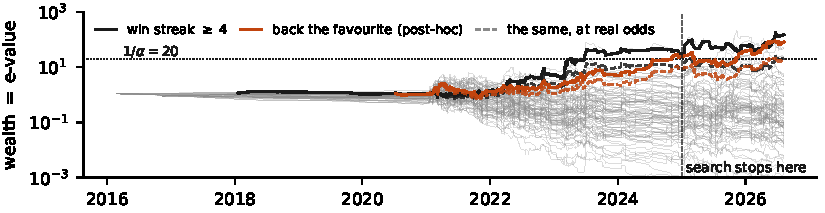
\includegraphics[width=\textwidth]{figs/continuation.pdf}
\caption{Wealth as a function of calendar time for every pre-registered segment (grey) and the two the analysis singled out (coloured). The dashed line is where the search stopped and the replication window began. A fixed-$n$ analysis must start a new test to the right of it; a test martingale does not.}
\label{fig:cont}
\end{figure}

\section{``Failed to replicate'' and ``not yet'' are different findings}

The original analysis froze its discovery window, selected the streak segment, and ran a fresh fixed-$n$ test on 2025--26. That test returned $p=0.30$ and was reported, correctly under its own logic, as a failure to replicate. It is the only move a fixed-$n$ design has: the second window buys a second test and nothing carries over.

On the wealth scale the same $110$ bouts read differently. The segment's log-growth in the replication window is $+0.0143$ nats per bout --- statistically indistinguishable from, and in fact slightly above, its discovery-window rate. The e-value accumulated there is $4.81$: real evidence, short of $1/\alpha=20$. At that growth rate, crossing needs $210$ bouts; $110$ have arrived. The finding is not refuted. It is $100$ bouts --- roughly eighteen months of cards --- from a decision, and an e-process lets one simply keep multiplying rather than choose a stopping time in advance (Figure~\ref{fig:cont}). We report the pre-split wealth ($e=31.4$) but do not claim it: that is the window in which the segment was chosen.

The effect is stable across the five walk-forward seeds the pool carries (e-values $56.2$ to $150.9$, all above $1/\alpha$), which the $q$-value machinery had no natural place to put.

\section{Pricing the freedom a post-hoc rule used}
\label{sec:posthoc}

\begin{figure}[t]
\centering
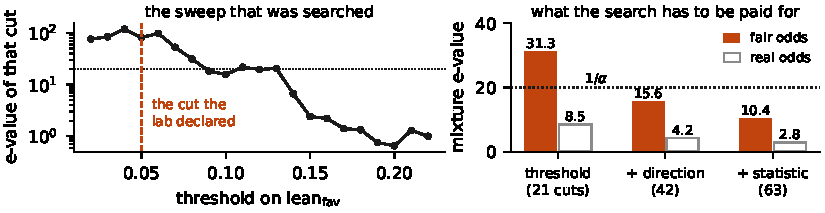
\includegraphics[width=\textwidth]{figs/posthoc.pdf}
\caption{Left: the e-value of each threshold on the model's lean toward the book's favourite. The declared cut at $0.05$ was chosen after this shape was visible. Right: a mixture martingale over progressively more of the freedom the search actually had. The finding survives paying for the threshold and does not survive paying for the direction.}
\label{fig:posthoc}
\end{figure}

The largest effect in the original analysis is not a segment but a direction: where the model gives the book's favourite \emph{more} than the book does, flat-staking that favourite returned $+11.5\%$ over $281$ bets across $163$ events. The analysis declared this post-hoc and said so --- the cut at $\mathrm{lean}\ge 0.05$ was chosen after seeing that the sweep was positive from $0.02$ to $0.22$ and peaked at $0.13$. A fixed-$n$ framework has no principled penalty for that.

A mixture martingale has one, and it is a price fixed in advance rather than argued after: each threshold's wealth process is a martingale starting at $1$, so any convex combination is too, and the search is paid for by the prior mass not placed on the winner. The maximum over thresholds is $118.99$ and is not a valid e-value. The uniform mixture over the $21$ cuts is $e=31.3$, which clears $1/\alpha$. Widening the family to the $21$ cuts the search could also have taken in the opposite direction gives $e=15.6$, which does not. Adding the other disagreement statistic available on the same frame gives $10.4$.

We regard the ladder, not any rung, as the result. It converts ``this was post-hoc'' from a caveat into a quantity: this finding can absorb the threshold search and cannot absorb the threshold search plus the choice of direction. We are not aware of a fixed-$n$ analysis that can state the boundary that precisely.

\section{What the sequential instrument needs}
\label{sec:planning}

Replacing the minimum detectable effect with a growth rate makes project planning a calculation rather than a verdict. Against a true $3$ pp edge simulated on this pool's own price distribution, the half-Kelly bet grows at $0.00166$ nats per bout and reaches $e=1/\alpha$ in ${\sim}1{,}800$ bouts; the paired log-loss test needs ${\sim}5{,}346$ at $80\%$ power. At $5$ pp the figures are $648$ and $1{,}902$. The sequential test is roughly $3\times$ cheaper in fights, not because it is more powerful per observation, but because a paired contrast on a slice discards most of what each bout carries.

Anytime-validity is not free, and the honest comparison says so. For the directional rule, the cluster bootstrap gives a $95\%$ interval on ROI of $[+2.2\%, +20.4\%]$ --- valid at the one $n$ at which the analysis stopped, which it chose after watching the number. A hedged betting confidence sequence, valid at every $n$ simultaneously, gives $[-5.3\%, +22.9\%]$ and does not exclude zero.

\section{Limitations}
\label{sec:limits}

The stake is a free choice. Fractional Kelly at $0.25/0.5/1.0$ gives $e = 26.0/150.9/115.3$ on the streak segment, and a predictable plug-in that learns the multiplier from past bouts only --- so not a choice at all --- settles at $c=0.70$ and $e=63.1$. Every variant clears $1/\alpha$; the conclusion is not the fraction.

Boosting e-BH \citep{wang2022} would recover power, but it requires the null distribution of each e-value, which a composite martingale null does not supply. Pre-specified weights across the nine declared families are a better route and were not pre-specified.

Three contaminations are inherited from the underlying pool and were sized there: the served model carries an age correction whose shipping decision used data inside the replication window; the model's hyperparameters were tuned on a window the pool later scores ($122$ of $1{,}191$ discovery bouts); and one derived rating is not fully point-in-time, contaminating $21.9\%$ of pool bouts, worth $0.0011$ nats. Each is small and each moves the reported numbers in the unfavourable direction if removed.

Finally, this is one sport, one book, and one model. The construction generalises to any forecaster audited against a market price; the numbers do not.

\bibliographystyle{plainnat}
\begin{thebibliography}{9}
\bibitem[Benjamini and Yekutieli(2001)]{benjamini2001} Y.~Benjamini and D.~Yekutieli. The control of the false discovery rate in multiple testing under dependency. \emph{Annals of Statistics}, 29(4):1165--1188, 2001.
\bibitem[Gr\"unwald et al.(2024)]{grunwald2024} P.~Gr\"unwald, R.~de~Heide, and W.~Koolen. Safe testing. \emph{Journal of the Royal Statistical Society: Series B}, 86(5):1091--1128, 2024.
\bibitem[Prigodskii(2026)]{vertexlab} R.~Prigodskii. Where does the model beat the book --- 87 slices, one survivor. Technical report, \textsc{Vertex MMA}, 2026.
\bibitem[Ramdas et al.(2023)]{ramdas2023} A.~Ramdas, P.~Gr\"unwald, V.~Vovk, and G.~Shafer. Game-theoretic statistics and safe anytime-valid inference. \emph{Statistical Science}, 38(4):576--601, 2023.
\bibitem[Shafer(2021)]{shafer2021} G.~Shafer. Testing by betting: a strategy for statistical and scientific communication. \emph{Journal of the Royal Statistical Society: Series A}, 184(2):407--431, 2021.
\bibitem[Wang and Ramdas(2022)]{wang2022} R.~Wang and A.~Ramdas. False discovery rate control with e-values. \emph{Journal of the Royal Statistical Society: Series B}, 84(3):822--852, 2022.
\bibitem[Waudby-Smith and Ramdas(2024)]{wsr2024} I.~Waudby-Smith and A.~Ramdas. Estimating means of bounded random variables by betting. \emph{Journal of the Royal Statistical Society: Series B}, 86(1):1--27, 2024.
\end{thebibliography}

\end{document}
